\section{}
\[
H(s)=\frac{-1000}{(s+1)(s+100)}\,.
\]
\subsection{Bode-Diagramm}
\begin{center}
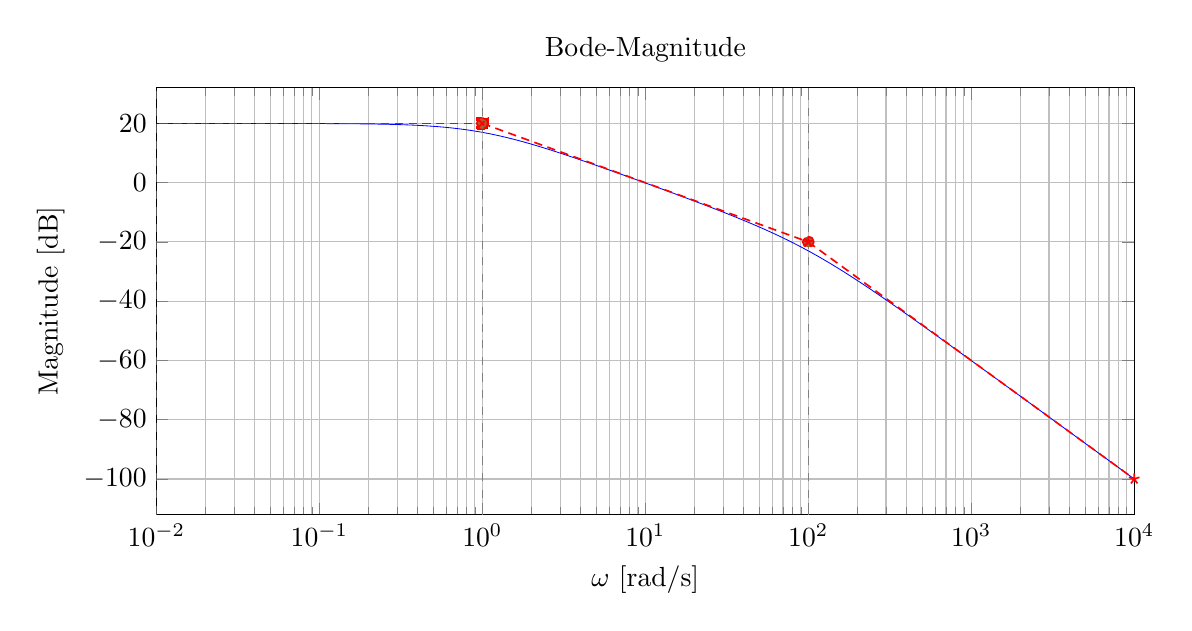
\begin{tikzpicture}
\begin{semilogxaxis}[
  width=14cm,height=7cm,
  xmin=1e-2,xmax=1e4,
  ytick distance=20,
  xlabel={$\omega$ [rad/s]},
  ylabel={Magnitude [dB]},
  grid=both,
  title={Bode-Magnitude}
]
\addplot[
  domain=1e-3:1e4,
  samples=800,
  mark=none,
  line width=0.3pt,
  blue
] {60 - 20*ln(sqrt(1 + x^2))/ln(10) - 20*ln(sqrt(10000 + x^2))/ln(10)};
\addplot+[domain=1e-3:1,samples=2,dashed,dash pattern=on 3pt off 2pt,line width=0.6pt,red] {20};
\addplot+[domain=1:1e2,samples=2,dashed,dash pattern=on 3pt off 2pt,line width=0.6pt,red] {20 - 20*ln(x)/ln(10)};
\addplot+[domain=1e2:1e4,samples=2,dashed,dash pattern=on 3pt off 2pt,line width=0.6pt,red] {-20 - 40*ln(x/100)/ln(10)};
\draw[gray,dashed] (rel axis cs:0,0) -- (rel axis cs:0,1);
\draw[gray,dashed] (axis cs:1,\pgfkeysvalueof{/pgfplots/ymin}) -- (axis cs:1,\pgfkeysvalueof{/pgfplots/ymax});
\draw[gray,dashed] (axis cs:100,\pgfkeysvalueof{/pgfplots/ymin}) -- (axis cs:100,\pgfkeysvalueof{/pgfplots/ymax});
\node[gray,anchor=south east] at (axis cs:1,\pgfkeysvalueof{/pgfplots/ymax}) {\scriptsize Pol $\omega_p=1$};
\node[gray,anchor=south east] at (axis cs:100,\pgfkeysvalueof{/pgfplots/ymax}) {\scriptsize Pol $\omega_p=100$};
\end{semilogxaxis}
\end{tikzpicture}
\vspace{6mm}
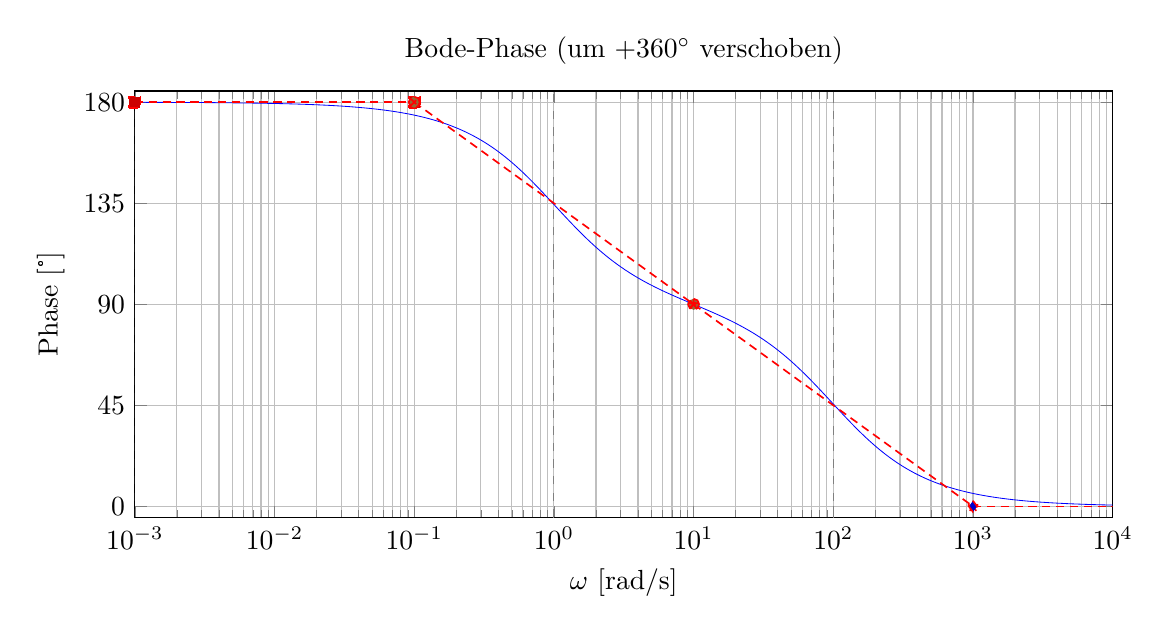
\begin{tikzpicture}
\begin{semilogxaxis}[
  width=14cm,height=7cm,
  xmin=1e-3,xmax=1e4,
  ymin=-5,ymax=185,
  ytick distance=45,
  xlabel={$\omega$ [rad/s]},
  ylabel={Phase [°]},
  grid=both,
  title={Bode-Phase (um $+360^\circ$ verschoben)}
]
\addplot[
  domain=1e-3:1e5,
  samples=800,
  mark=none,
  line width=0.3pt,
  blue
] {180 - atan(x) - atan(x/100)};
\addplot+[domain=1e-3:1e-1,samples=2,dashed,dash pattern=on 3pt off 2pt,line width=0.6pt,red] {180};
\addplot+[domain=1e-1:1e1,samples=2,dashed,dash pattern=on 3pt off 2pt,line width=0.6pt,red] {135 - 45*ln(x)/ln(10)};

\addplot+[domain=1e1:1e3,samples=2,dashed,dash pattern=on 3pt off 2pt,line width=0.6pt,red]{45 - 45*ln(x/100)/ln(10)};
\addplot+[domain=1e3:1e5,samples=2,dashed,dash pattern=on 3pt off 2pt,line width=0.6pt,red]{0};
\draw[gray,dashed] (rel axis cs:0,0) -- (rel axis cs:0,1);
\draw[gray,dashed] (axis cs:1,\pgfkeysvalueof{/pgfplots/ymin}) -- (axis cs:1,\pgfkeysvalueof{/pgfplots/ymax});
\draw[gray,dashed] (axis cs:100,\pgfkeysvalueof{/pgfplots/ymin}) -- (axis cs:100,\pgfkeysvalueof{/pgfplots/ymax});
\node[gray,anchor=south east] at (axis cs:1,\pgfkeysvalueof{/pgfplots/ymax}) {\scriptsize Pol $\omega_p=1$};
\node[gray,anchor=south east] at (axis cs:100,\pgfkeysvalueof{/pgfplots/ymax}) {\scriptsize Pol $\omega_p=100$};
\end{semilogxaxis}
\end{tikzpicture}
\end{center}
\newpage

\subsection{Erklärung}
\begin{description}[leftmargin=1.2em,labelsep=.6em,font=\bfseries]

\item[1. Normalform herstellen.]
\[
H(s)=\frac{-1000}{(s+1)(s+100)}
= \frac{K_0}{(1+sT_{p1})(1+sT_{p2})}
\]
mit
\[
K_0=-10,\quad r=0,\quad T_{p1}=1,\quad T_{p2}=\tfrac{1}{100}.
\]
\[
\underline{F}_1(s)=\frac{1}{1+sT_{p1}}=\frac{1}{1+s},\qquad
\underline{F}_2(s)=\frac{1}{1+sT_{p2}}=\frac{1}{1+\tfrac{s}{100}}.
\]
Konstantes Vorzeichen \(K_0<0\): Phasenoffset \(\pm180^\circ\) (hier Darstellung um \(+360^\circ\) verschoben).

\item[2. Eckfrequenzen bestimmen und sortieren.]Die $\omega$-Eckfrequenzen lassen sich aus den $T_n$'s bestimmen und müssen anschließend sortiert werden:
\[
\omega_{p1}=\frac{1}{T_{p1}}=1\,\mathrm{rad/s},\qquad \omega_{p2}=\frac{1}{T_{p2}}=100\,\mathrm{rad/s},\qquad \omega_{p1}<\omega_{p2}.
\]

\item[3. Startpunkt des Amplitudengangs festlegen (Geradennäherung).]
\[
\omega_{\min}=\omega_{p1}=1,\quad
F_{\mathrm{dB}}(\omega_{\min})=20\log_{10}\!\big(|K_0\underline{F}_{ges}^*(0)|\,\omega_{\min}^{\,r}\big)=20\log_{10}10=20\,\mathrm{dB}.
\]
Unser Ankerpunkt ist: \(20\,\mathrm{dB}\) bei \(\omega=1\).

\item[4. Verlauf links vom Startpunkt zeichnen.]
Für \(\omega<\omega_z\) bleibt die Amplituden-Asymptote bei \(20\,\mathrm{dB}\) konstant (Anfangssteigung \(r\cdot 20 \,\mathrm{dB}=0\)). Zeichne eine waagrechte Gerade links von der kleinsten Eckfrequenz.

\item[5. Steigungswechsel an den Eckfrequenzen eintragen.]
Ab \(\omega=1\): \(-20\,\mathrm{dB/dec}\) (einfacher Pol).
Ab \(\omega=100\): zusätzl. \(-20\,\mathrm{dB/dec}\) \(\Rightarrow\) insgesamt \(-40\,\mathrm{dB/dec}\).
Geradennäherungen:
\[
|H(j\omega)|_{\mathrm{dB}}\approx
\begin{cases}
20,& \omega\le 1,\\
20-20\log_{10}\omega,& 1<\omega\le 100,\\
-20-40\log_{10}(\omega/100),& \omega\ge 100.
\end{cases}
\]

\item[6. Eckabrundungen korrekt berücksichtigen.]
Bei jedem einfachen Pol: \(-3\,\mathrm{dB}\) am Knick.
\[
|H(j1)|_{\mathrm{dB}}=20-10\log_{10}2\approx 17\,\mathrm{dB},\qquad
|H(j100)|_{\mathrm{dB}}=-20-10\log_{10}2\approx -23\,\mathrm{dB}.
\]

\item[7. Phasenstartwert festlegen.]
Wegen \(K_0<0\): Startphase \(-180^\circ + r\cdot90^\circ=-180^\circ\). Darstellung um \(+360^\circ\) verschoben \(\Rightarrow\) \(+180^\circ\) für \(\omega\ll 0.1\).

\item[8. Phasenänderung durch die Polglieder eintragen.]
Jeder einfache Pol: \(-90^\circ\) über je eine Dekade.
Näherung (verschobene Darstellung):
\[
\varphi(\omega)\approx
\begin{cases}
180^\circ,& \omega\le 0.1,\\
135^\circ-45^\circ\log_{10}\omega,& 0.1<\omega<10,\\
45^\circ-45^\circ\log_{10}(\omega/100),& 10<\omega<1000,\\
0^\circ,& \omega\ge 1000.
\end{cases}
\]

\item[9. Grenzwerte und Konsistenz prüfen.]
DC: \(|H(0)|=10\Rightarrow 20\,\mathrm{dB}\); Phase \(-180^\circ\) (hier als \(+180^\circ\) gezeigt).
HF: \(|H(j\omega)|\sim 10/\omega^2\Rightarrow -40\log_{10}(\omega/100)-20\,\mathrm{dB}\). 
Pol-/Nullzählung bestätigt die Endphase: \(m=0\), \(n=2\Rightarrow (m-n)\cdot 90^\circ=-180^\circ\); plus negatives \(K_0\) \(\Rightarrow\) zusätzlich \(-180^\circ\); gesamte \(-360^\circ\equiv 0^\circ\) (mod \(360^\circ\)).

\end{description}

\subsubsection*{Stückweise Näherungen (für die Skizze)}
\[
|H(j\omega)|_{\mathrm{dB}}\approx
\begin{cases}
20,& \omega\ll 1,\\[2pt]
20-10\log_{10}2,& \omega=1,\\[2pt]
20-20\log_{10}\omega,& 1\ll\omega\ll 100,\\[2pt]
-20-10\log_{10}2,& \omega=100,\\[2pt]
-20-40\log_{10}(\omega/100),& \omega\gg 100,
\end{cases}
\]\[
\varphi(\omega)\ (\text{um }+360^\circ)\approx
\begin{cases}
180^\circ,& \omega\le 0.1,\\[2pt]
135^\circ-45^\circ\log_{10}\omega,& 0.1<\omega<10,\\[2pt]
45^\circ-45^\circ\log_{10}(\omega/100),& 10<\omega<1000,\\[2pt]
0^\circ,& \omega\ge 1000.
\end{cases}
\]

\newpage